\documentclass{thesisKGI}

  %------------------- TITULNÍ STRANA ------------------- 

  \title{SYNCHRONIZACE A REPLIKACE GEODAT V PROSTŘEDÍ ESRI PLATFORMY}
  \author{Markéta SOLANSKÁ}
  \thesistype{Magisterská práce}
  \advisor{doc. RNDr. Vilém Pechanec, Ph.D.}

  \bibliographystyle{csplainnat} %styl citací


  \begin{document}
    \sloppy       %lepší hlídání přetékajících řádků
    \maketitle    %vložení titulní strany

    %------------------------------------------------------------------------- ČESTNÉ PROHLÁŠENÍ

    %vložení prohlášení, třída se sama postará o tvorbu nové stránky a vloží pod text řádek s datumem a jménem
    \begin{declaration}
      \textbf{Čestné prohlášení}

      Prohlašuji, že jsem magisterskou práci magisterského studia oboru Geoinformatika vypracovala samostatně pod vedením RNDr. Viléma Pechance, Ph.D.

      Všechny použité materiály a zdroje jsou citovány s ohledem na vědeckou etiku, autorská práva a zákony na ochranu duševního vlastnictví.

      Všechna poskytnutá i vytvořená digitální data nebudu bez souhlasu školy poskytovat.
    \end{declaration}

    %------------------------------------------------------------------------- PODĚKOVÁNÍ
    
    %poděkování, pokud nějaké chcete uvést, jinak lze tuto sekci smazat
    \begin{dedication}

      Děkuji vedoucímu práce doc. RNDr. Vilému Pechancovi, Ph.D. za podněty a připomínky při vypracování práce.

      Děkuji také konzultantu Tomáši Vondrovi za pomoc při pochopení a praktickém použití databázového serveru PostgreSQL, za jeho rady a podněty, stejně tak jako i jeho kolegovi Pavlovi Stěhule.

      Dále děkuji konzultantům Boudewijn van Leeuwen a Zalan Tobak z University of Szeged za připomínky a podněty k této práci. 
      \vspace{4em}
    \end{dedication}

    %------------------------------------------------------------------------- NASTAVENÍ POČÍTADLA, ZKRATKY
    
    \setcounter{page}{5}          %nastavení počítadla stránek na správnou hodnotu
    \makeTableOfContent{3}        %vložení obsahu, standardně se používají 3 úrovně

    \makeGlossary                 %formát v nemž se vkládají zkratky, vlouží se pouze ty, které budou použity v textu. v textu vkládáme zkratku pomocí příkazu \gls{DTM}
    %vložení seznamu zkratek, smazat, pokud není třeba
      \newglossaryentry{CAD}{name=CAD, description={Computer Aided Design}}
      \newglossaryentry{GIT}{name=GIT, description={geoinformační technologie}}
      \newglossaryentry{SQL}{name=SQL, description={Structured Query Language}}

    %------------------------------------------------------------------------- ÚVOD
    %protože je Úvod nečíslovaný je potřeba ho manuálně vložit do obsahu
    \addcontentsline{toc}{section}{ÚVOD}
    \section*{Úvod}
      Dnešní trend je ukládat a ponechávat stále více dat pouze v digitální podobě. Mnoho dokumentů už se vůbec netiskne do papírové podoby, což podporuje i trend e\-le\-ktro\-nic\-kých schránek a podpisů. S přibývajícím množstvím dat je však třeba řešit komplikace, které informace uložené pouze v elektronické podobě přinášejí. Počítačoví experti řeší například otázky, kam ukládat tak velké množství dat, jak data efektivně aktualizovat, jak zabránit poškození dat ať už způsobených lidským faktorem či chybou hardware. V případě, že se poškodí disk, můžeme často během okamžiku přijít o~všechna data, někdy však pro ztrátu dat stačí pouze stisknout tlačítko na klávesnici.

Dnes je běžné, že má každý hned několik internetových účtů pro přihlášení do banky, pojišťovny, různých internetových obchodů, či sociální sítě. Často však, například z důvodu přetížení, nastávají problémy s pomalým připojením nebo úplnou nedostupností zvolené služby. I to jsou problémy, které velké množství dat a vysoký počet uživatelů přináší. Jak tedy pracovat s těmito objemy, jak zabránit komplikacím, které mohou poškodit či zcela zničit celou dosavadní práci, a~jak zrychlit celý proces práce s daty? 

Řešením velkého počtu výše uvedených problémů může být ukládaní dat do databáze a jejich následná replikace. Replikací je myšlena pokročilá funkcionalita, která zajišťuje kopii dat na více serverů. Nabízí ji většina dnešních databázových serverů, zajišťuje větší robustnost databáze a vysokou dostupnost dat. Replikaci lze využít ve všech odvětvích, která pracují s daty. Výjimkou není ani geoinformatika, která často pracuje s~velkými objemy dat, které nesou informaci o geografické poloze. Právě reprezentace geografické polohy, skrze textový zápis souřadnic daných bodů, může způsobit razantní zvýšení objemu dat. U webových map se musí řešit velký počet dotazů do databáze, protože například každé posunutí výřezu či přiblížení, resp. oddálení výřezu mapy, je samostatným dotazem, který musí kapacita serveru zvládat. Například pokud bude uživatel procházet plánovanou 100km trasu posouváním výřezu mapy po 10~km, může to serveru způsobit velkou zátěž.

Data středně velkého až velkého projektu je vhodnější ukládat do databáze než jiných formátů typu shapefile, GML nebo obyčejného tabulkového procesoru. Nabízí nám to sofistikované uložení dat, propojení jednotlivých vrstev a připojení atributů ke geometrii, snadnou přenostitelnost dat i efektivní vyhledávání. Replikace samotná se poté využívá pro zajištění kopie dat a následnou aktualizaci změn, která v databázi nastanou. 

Replikaci ocení uživatelé pracující na společném projektu, distribuovaná pra\-co\-viš\-tě i společnosti s velkým množstvím důležitých dat, jejichž dostupnost je rozhodující pro jejich fungování. Dobrým příkladem využitelnosti replikace a synchronizace je také nový trend využívání offline aplikací v mobilních telefonech. Databáze se vždy replikuje do mobilního telefonu, kde může fungovat offline a vždy, když se klient připojí na internetovou síť, aplikace zkontroluje zda není na serveru novější verze databáze a pokud ano, zkopíruje pouze změny, které proběhly od poslední aktualizace. Databázové systémy nabízí širokou škálu nastavení, která umožňuje replikaci přizpůsobit danému řešení.



    %------------------------------------------------------------------------- CÍLE PRÁCE
    %každou kapitolu je třeba začít na nové stránce
    \newpage
    \section{CÍLE PRÁCE}
      
      Cílem diplomové práce je provést rešerši a na jejím základě
      prakticky otestovat proces synchronizace a replikace geodat, které
      se dnes objevují napříč platformou Esri. V teoretické části práce
      bude detailně analyzován proces synchronizace a replikace ve všech
      možných variantách (jednosměrná, dvousměrná, synchronní,
      asynchronní, ...) a popsány prostředky, které se na platformě Esri k
      těmto procesům využívají. Rozbor zahrne celé portfólio produktů od
      desktop řešení, přes možnosti ArcGIS serveru až po cloudový ArcGIS
      online. Budou popsány možnosti, požadavky a předpoklady pro úspěšnou
      realizaci.

      V praktické části, nad existujícími katedrálními daty, dojde k
      praktickému testování těchto procesů na předem připraveném
      testovacím prostředí. Postupnými opakovanými procesy budou sledovány
      dílčí parametry procesu (rychlost procesu, úplnost, chybovost,
      podporované formáty). Vyjde se z primárně podporovaného databázového
      stroje SQL Server, který bude konfrontován s možnosti dalšího
      podporovaného systému PostgeSQL.

      Můj jeden odstaveček - něco jako - jak vidím vlastní přínos do tématu. 


    %------------------------------------------------------------------------- POUŽITÉ METODY A POSTUPY PRÁCE
    \newpage
    \section{POUŽITÉ METODY A POSTUPY PRÁCE}
       \subsection{Obrázky}

    %ukázka zápisu kódu pro obrázek
    %parametr H říká že to bude přímo na tom místě kde je v textu...více http://en.wikibooks.org/wiki/LaTeX/Floats,_Figures_and_Captions
    \begin{figure}[H]
      \centering
      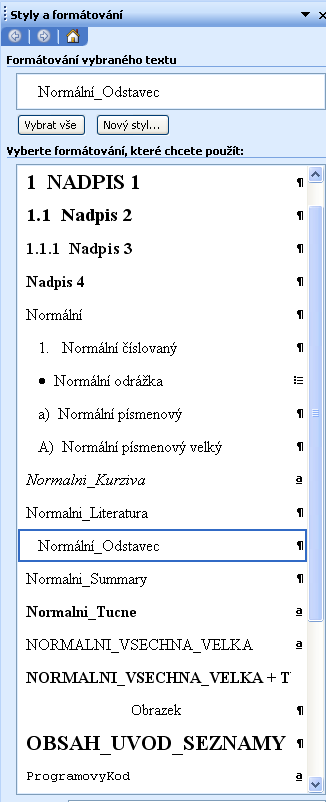
\includegraphics[width=0.2\textwidth]{./obrazky/obrazek_1.png}
      \caption {Styly (převzato z: \cite{Celikyilmaz2009})}
      \label{fig:44}
    \end{figure}

    %ukázka odkazu na zkratky a obrázek
    \Gls{GIT} \Gls{CAD} bla bla bla \odkazObrazek{fig:44}. Pokud chceme uvést překlad z angličtiny můžeme to udělat takto \transl{english words}.

    %dají se dělat i složené obrázky
    \begin{figure}
        \centering
        \begin{subfigure}[b]{0.45\textwidth}
          \centering
          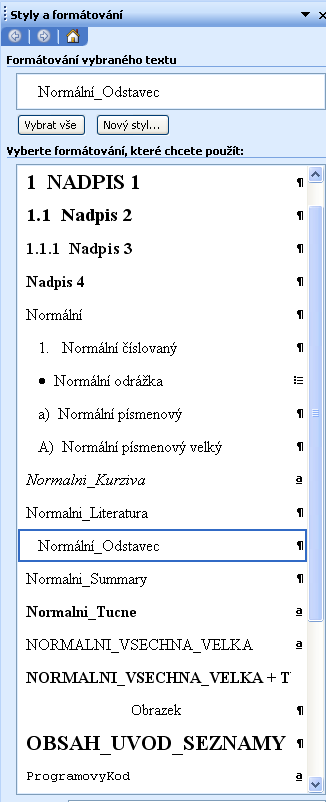
\includegraphics[width=\textwidth]{./obrazky/obrazek_1.png}
          \caption{Cena za metr čtvereční bytů v Londýně (převzato z:\cite{Fotheringham2002})}
          \label{fig2.1}
        \end{subfigure}%
        \quad %add desired spacing between images, e. g. ~, \quad, \qquad etc.
          %(or a blank line to force the subfigure onto a new line)
        \begin{subfigure}[b]{0.45\textwidth}
          \centering
          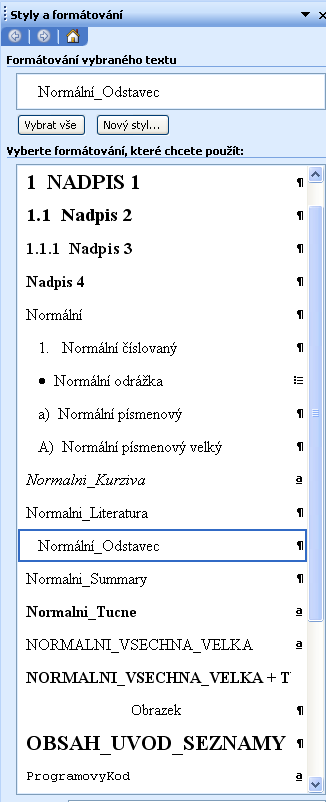
\includegraphics[width=\textwidth]{./obrazky/obrazek_1.png}
          \caption{Obsah zinku v půdě (převzato z:\cite{Hengl2009})}
          \label{fig2.2}
        \end{subfigure}
        \caption{Povrch socioekonomického (a) a fyzickogeografického (b) ukazatele}
        \label{fig2}
    \end{figure}

    \begin{table}[h]
    \caption {Ukázková tabulka}
    \label{tab1}
    \centering
      \begin{tabular}{ |l|l|l| }
        \hline
        \multicolumn{3}{ |c| }{Team sheet} \\
        \hline
        Goalkeeper & GK & Paul Robinson \\ \hline
        \multirow{4}{*}{Defenders} & LB & Lucus Radebe \\
        & DC & Michael Duberry \\
        & DC & Dominic Matteo \\
        & RB & Didier Domi \\ \hline
        \multirow{3}{*}{Midfielders} & MC & David Batty \\
        & MC & Eirik Bakke \\
        & MC & Jody Morris \\ \hline
        Forward & FW & Jamie McMaster \\ \hline
        \multirow{2}{*}{Strikers} & ST & Alan Smith \\
        & ST & Mark Viduka \\
        \hline
      \end{tabular}
    \end{table}

    Odkaz na tabulku pak vytvoříme takto: \odkazTabulka{tab1}.

    \begin{equation}
    \label{eq1}
    c = \sqrt{a^2 + b^2}
    \end{equation}

    Vzorce pak odkazujeme \odkazVzorec{eq1}. 

    Citace se dají dělat buď jako \citep{Talasova2003} nebo \cite{Talasova2003}.



    
    %------------------------------------------------------------------------- TEORETICKÁ VÝCHODISKA
    \newpage
    \section{TEORETICKÁ VÝCHODISKA}
    
    %------------------------------------------------------------------------- VÝSLEDKY
    \newpage
    \section{VÝSLEDKY}

    %------------------------------------------------------------------------- DISKUZE
    \newpage
    \section{DISKUZE}

    %------------------------------------------------------------------------- ZÁVĚR
    \newpage
    \section{ZÁVĚR}

    %------------------------------------------------------------------------- LITERATURA
    \newpage
    \addcontentsline{toc}{section}{LITERATURA}
    %\makeBibliography{literatura}
    \bibliography{literatura}

    %------------------------------------------------------------------------- ILUSTRACE
    \newpage
    \addcontentsline{toc}{section}{SEZNAM ILUSTRACÍ}
    \section*{SEZNAM ILUSTRACÍ/TABULEK}

    %------------------------------------------------------------------------- SUMMARY
    \begin{summary}
      There is summary of all aims, methods and results in this chapter.
      Summary is not only translation of chapter Závěr. There is more
      information from chapters Cíle, Výsledky and Diskuze. Number of
      pages of Summary chapter is two at least. The style is Normalni
      Summary. Language is set to Angličina(Velká Británie) for automatic
      spell check. Do not use language Angličtina(USA). 
    \end{summary}

    %------------------------------------------------------------------------- PŘÍLOHY
    \newpage
    \vspace*{180pt}
    \begin{center}
      {\Large\textbf{PŘÍLOHY}}
    \end{center}
    \vspace*{\fill}

    \newpage
    \addcontentsline{toc}{section}{PŘÍLOHY}
    \section*{SEZNAM PŘÍLOH}
    \textbf{Volné přílohy}

    Příloha 1 CD \newline
    \newline
    \textbf{Popis sktruktury CD}

      Adresáře a soubory:

        - složka se skripty

        - web - webová stránky jako doplněk k diplomové práci

        - Solanska\_dp.pdf - text diplomové práce

    \vspace*{\fill}

  \end{document}
